\documentclass[a4paper]{article}

\usepackage[english]{babel}
\usepackage[utf8]{inputenc}
\usepackage{float}
\usepackage{amsmath}
\usepackage{graphicx}
\usepackage{subfigure}
\usepackage[colorinlistoftodos]{todonotes}

\title{\bfseries{COMP90016 -- Assignment 1 }}
\author{Haonan Li}

\date{\today}

\begin{document}
\maketitle

\section{Introduction}
\label{sec:introduction}

This assignment consists of three tasks. 

For the first task, we first build a k-mer index for a reference file, then aligned all reads from a FASTQ reads file using the index.

The second task is to investigate the runtime of the aligner build in task 1. In this task, we compare the speed of the new aligner with the naive aligner proposed in group assignment. In addition, we also evaluate the relation between size of k-mer and the alignment speed.

For the last task, we extend our algorithm to further investigate mismatches to the reference.

\section{Results \& Discussion}
\label{sec:experiment}
\subsection{Task 2}

\begin{table}[H]
	\centering
	\begin{tabular}{c|c|c|c|c|c|c|c}
		\hline
		k & 0 & 4 & 8 & 13 & 16 & 32 & 50 \\
		\hline
		ref1 & 24.43 & 18.98 & 1.76 & 1.48 & 1.40 & 1.04 & 0.51 \\
		\hline
		ref2 & 50.87 & 35.34 & 1.83 & 1.49 & 1.49 & 1.14 & 0.66 \\
		\hline
		ref3 & 80.54 & 52.65 & 1.91 & 1.56 & 1.47 & 1.22 & 0.78\\
		\hline
	\end{tabular}
	\caption{\label{tab:1}Time consuming for k-mer indexed alignment. (k=0, refers to  the naive aligner.)}
\end{table}

Table \ref{tab:1} shows the time consuming for k-mer aligner work on the given datasets. $K=0$ refers to the naive aligner proposed in group assignment. From these results, we find that new aligner is much more efficiently than the naive alignments.

The result is not surprised. Because the  complexity of naive Hamming distance aligner is $O(ngl)$, where $n$ is the number of reads, $g$ the length of the genome, and $l$ the length of the reads. But for indexed aligner, the complexity is O($nl^2+g$), here are theoretically analysis.

First assuming the length of k-mer is k, where $ k\ll l$, then for each read, we have $l-k$ k-mers and suppose for each k-mer, the number of indexed positions is p. So we need to compre $O((l-k)*l*p)$ times for each read. As $k\ll l$, $O(l-k)=O(l)$. Here, we have a complexity of $O(nl^{2}p)$. We normally assume that we can build a linear spaced index with constant number of positions for each k-mer,\footnote{Actually, if k is large enough, p will equals 1} and length of genome maybe very large, so we need to traverse it to build the index. Finally, the complexity is $O(nl^{2} + g)$.

Figure \ref{aa} shows new aligner's alignment time with the reference length. We change reference length from 0 to 5000 using ref3.fa, with every 15 one point. This figure indicates that time consuming changes linearly with reference length from 0 to 5000, 

Figure \ref{bb} shows new aligner's alignment time with the read length. We can identify it is a part of quadratic function.

Figure \ref{00} shows aligner's alignment time with k (the k-mer length), $k=0$ indicates the naive aligner's time. From which we find that when k is big enough. TIme consuming almost does not change with k.

Figure \ref{cc} is the visualization of two aligner's time comparison. We find that new aligner is faster then the naive aligner.
\begin{figure}[h]
	\centering
	\subfigure[Time consuming change with reference length]{
		\label{aa} 
		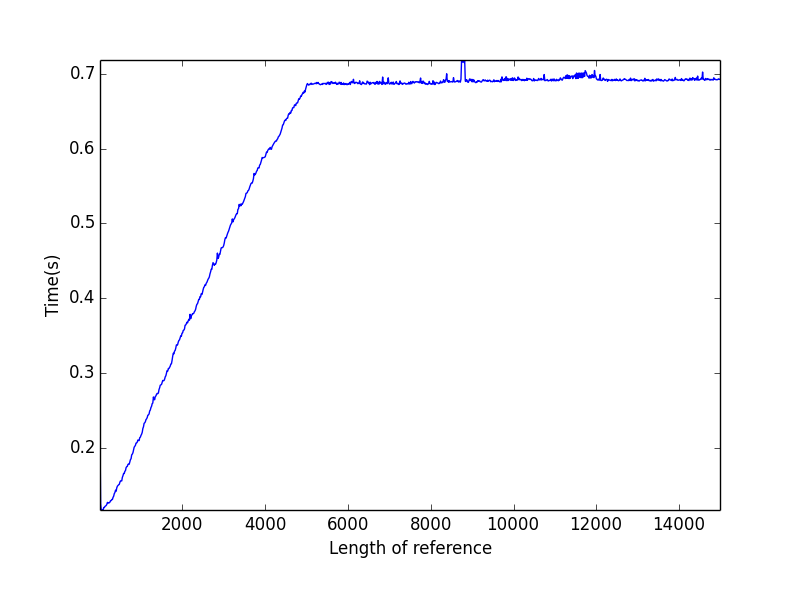
\includegraphics[width=0.45\textwidth]{time_ref_len.png}}
	\subfigure[Time comsuming change with read length]{
		\label{bb} 
		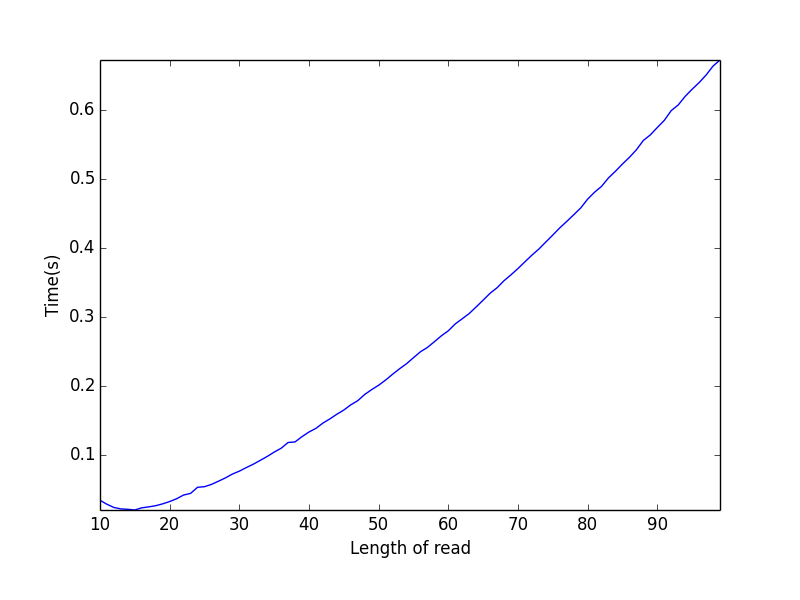
\includegraphics[width=0.45\textwidth]{time_read_len.png}}
	\subfigure[Time consuming change with k]{
		\label{00}
		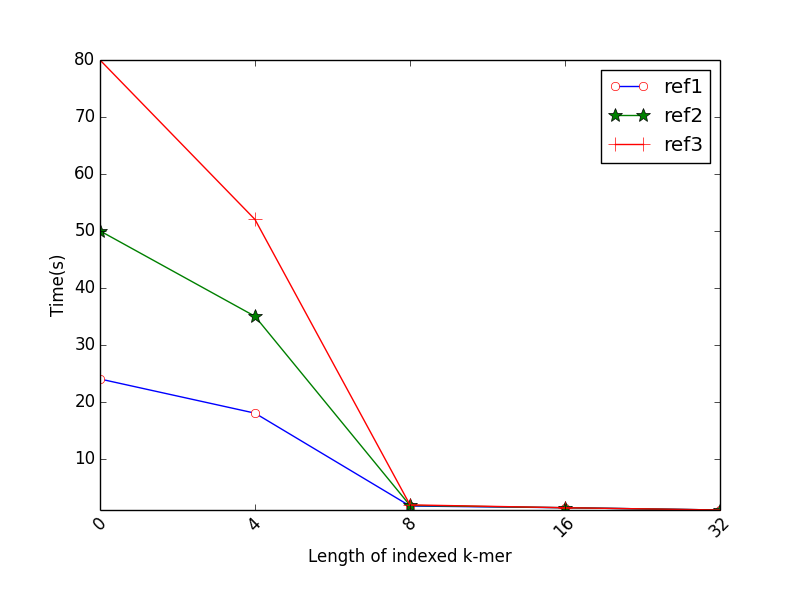
\includegraphics[width=0.45\textwidth]{align_time.png}}
	\subfigure[TIme consuming visulation of fixed k]{
		\label{cc} 
		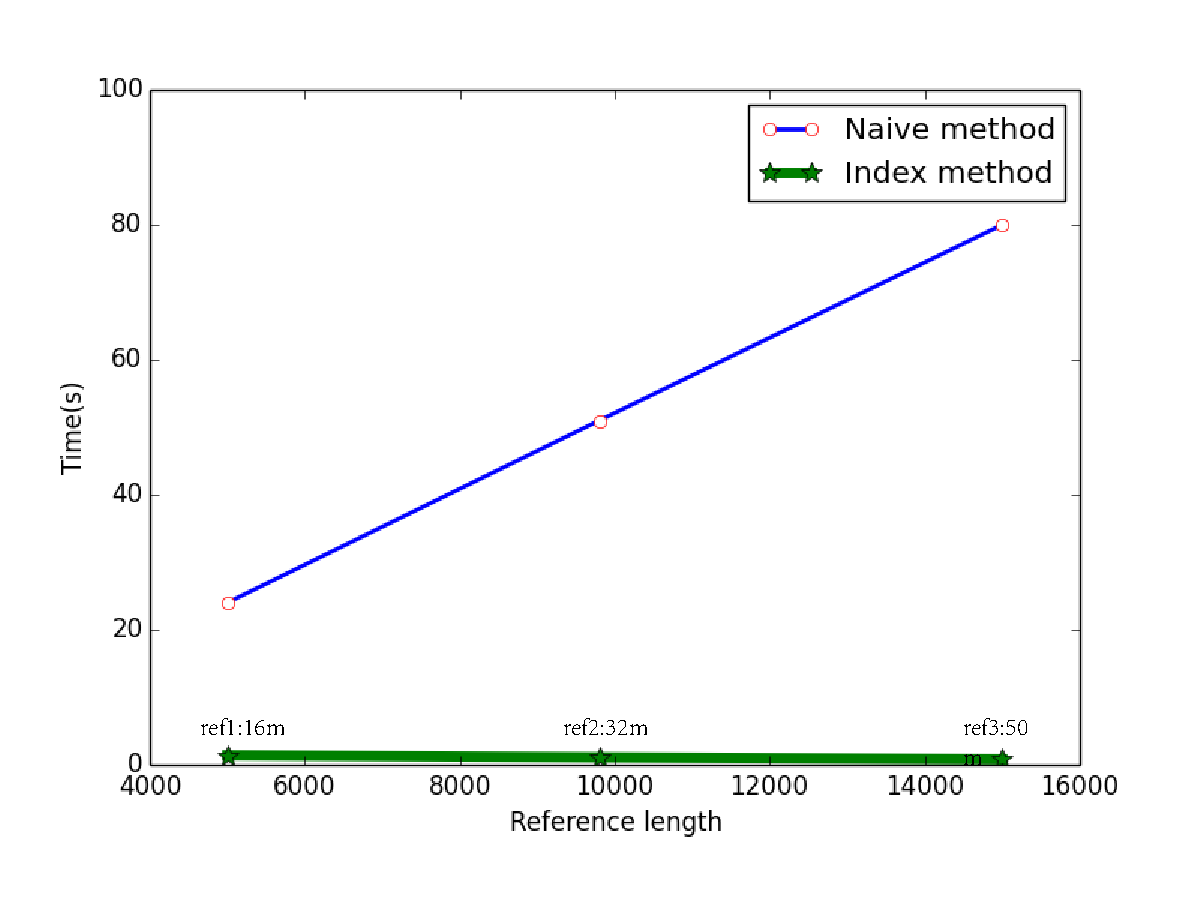
\includegraphics[width=0.45\textwidth]{align_vis.pdf}}
	\caption{Time sonsuming analysis.}
	\label{fig:time} 
\end{figure}

\subsection{Task 3}

Figure \ref{a}  shows the distribution of base quality scores of all the reads for each position, and Figure \ref{b} the distributions of quality scores of all mismatches for best alignment to the given reference ref1.fa  (also by position). 

Compare these two images, we find that the range of each position's quality score of two pictures are similar, which indicates even a position has a high average quality score or most quality scores of this position is high, mismatches occurred.  In addition, both of them shows that the middle position's quality score commonly higher than the start and end of the reads, this might because of the sequencing method.

However, no matter the upper quartile, lower quartile and median, two pictures show some differences. For most positions, the box of upper quartile to lower quartile of mismatched picture always lower than that for all reads. This might due to more low quality scores appear in the mismatched set.  Algorithm there are exceptions that median for mismatches upper than it for all reads, which might because the dataset is small. Besides, as the position varies form 1 to 100, the average quality score becomes lower, mismatches increase. This was reflected by the median lines that get closer to the bottom and even overlapped with it as the positions near to 100.

\begin{figure}[!htb]
	\centering
	\subfigure[All the reads for each position]{
		\label{a} 
		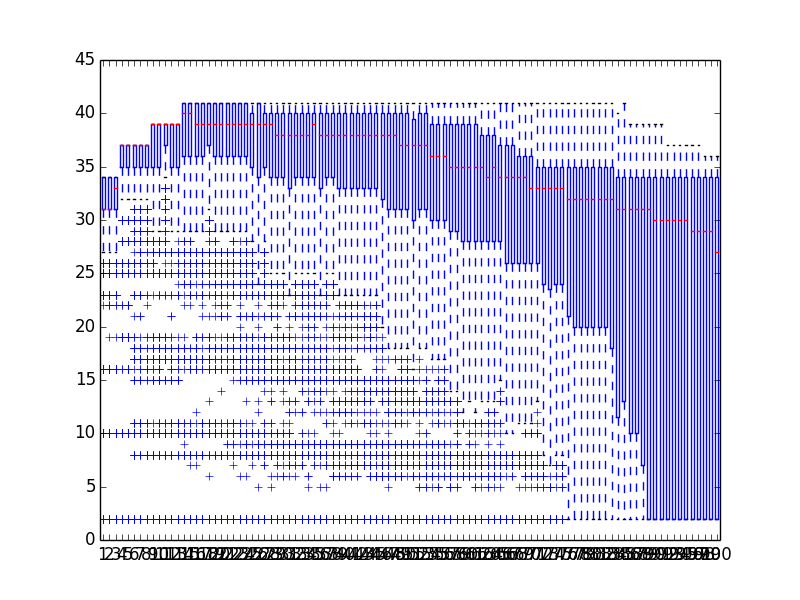
\includegraphics[width=0.47\textwidth]{base_qs.png}}
	\subfigure[All mismatches]{
		\label{b} 
		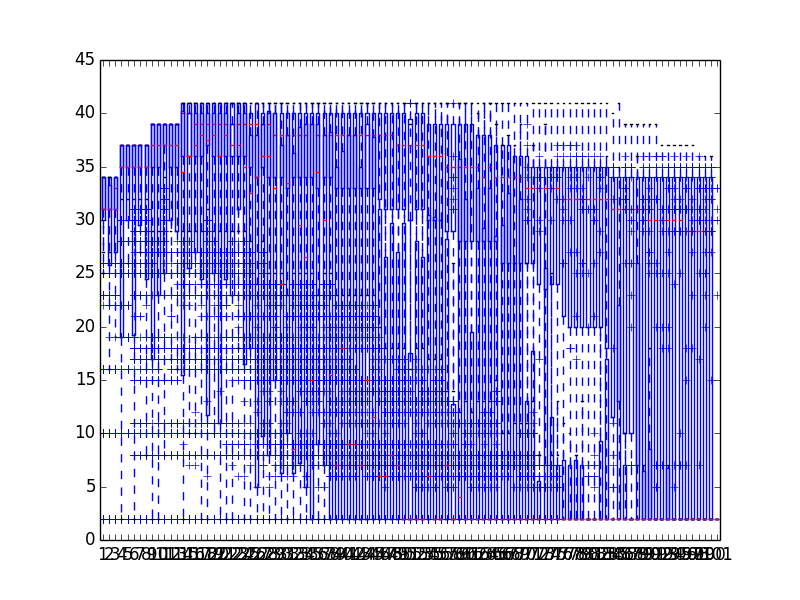
\includegraphics[width=0.47\textwidth]{mis_qs.png}}
	\caption{Distribution of base quality scores.}
	\label{fig:2} 
\end{figure}
 


%\begin{thebibliography}{9}
%\end{thebibliography}
\end{document}